\documentclass[12pt, a4paper]{article}
\usepackage[margin=2.5cm]{geometry}
\usepackage{xcolor}
\usepackage{todonotes}
\usepackage{amsthm, amsmath, ebproof}
\usepackage{algorithm}
\usepackage{algpseudocode}
\usepackage[colorlinks=true, 
            linkcolor=blue,
            citecolor=green,
            pdftitle={Master Thesis Proposal}]{hyperref}

\newcommand{\textrosu}[1]{\textcolor{red}{#1}}
\newcommand{\stodo}[2][]
{\todo[caption={#2}, size=\small, #1]{\renewcommand{\baselinestretch}{0.5}\selectfont#2\par}}

\title{Master Thesis}
\author{Certified Circuit Reconstruction for QBF}
\setlength{\parindent}{0pt}
\linespread{1.25}
\setlength{\marginparwidth}{2cm}


\newtheorem{theorem}{Theorem}[section]
\newtheorem{corollary}{Corollary}[theorem]
\newtheorem{claim}[theorem]{Claim}

\theoremstyle{definition}
\newtheorem{definition}[theorem]{Definition}
\newtheorem{example}[theorem]{Example}

\begin{document}

\maketitle
\tableofcontents
\newpage

\section{Introduction}



\subsection{Aim of the thesis}
\subsection{Related work}
\subsection{Work structure}



\section{Preliminary}

In this preliminary chapter, we are going to set the building blocks needed for later chapters without the need of prior knowledge. In all sections of this chapter, every definition will be accompanied by its respective example, and a corresponding illustration for each procedure.

A notion can have all sorts of definition, thus we shall include the citation for every introduced concept.

The structure of this chapter will be as follows: we start by introducing syntax and semantics for our formulas of interest, followed by a transformation of a generic formula in a conjunctive normal form. In plus, we present two proof systems for QBFs and show how an algorithm can solve a QBF. Lastly, we talk about types of format a QBF should be given in to be understood by a solver.

\subsection{QBF}

The quantified Boolean formula is an extension of the propositional Boolean formula with quantified variables. For example, $(x_1 \lor x_2 \land x_3) \to x_4$ is a propositional formula whilst $\forall x_1x_3 \exists x_2x_4(x_1 \lor x_2 \land x_3) \to x_4$ is the prior formula quantified.

Worth mentioning is that, every propositional formula can be represented as a QBF, by existentially quantified the variables, from $x_1 \lor x_2$ to $\exists x_1x_2 (x_1 \lor x_2)$.

In this section, the definition for QBF will be given in the prenex form, where all the quantification appear before a quantifier free formula named matrix. The matrix, as well, can be given in a special form, this will be conjunctive normal form. Any generic QBF can be transformed in the prenex conjunctive normal form. In this chapter, we will present only the transformation of the matrix in CNF in section \ref{pre:tseitin} using Tseitin transformation.

\begin{definition}[Literal \cite{handbook}]
    A \textbf{literal} is a Boolean variable $x$ or its negation $\overline{x}$. Let the function \textbf{var}$(l) = x$.
\end{definition}

\begin{example}
    In formula $(x \lor \overline{y} \land z)$ the literals are $\{ x, \overline{y}, z \}$. var$(\overline{y}) = y$. If we want the negation of the literal $l = \overline{y}$, we will have $\overline{l} = y$. Also, $x \lor \overline{y}$ is not a literal because it is the conjunction of two literals.
\end{example}

\begin{definition}[Clause \cite{handbook}]
    A \textbf{clause} is a disjunction of literals.
\end{definition}

\begin{example}
    $(x_1 \lor \overline{x_2} \lor x_3)$ is a clause. But $(y_1 \lor \overline{y_2} \land y_3)$ is not because it contains an and operator, neither $(z_1 \lor (\overline{z_2} \land z_3))$ because the second term is not a literal.
\end{example}

A clause can also be represented as a set, $(x_1 \lor \overline{x_2} \lor x_3)$ to $\{ x_1, \overline{x_2}, x_3 \}$. This representation is useful for computer programs due to its processing as a list.

\begin{definition}[Cube \cite{handbook}]
    A \textbf{cube} is a conjunction of literals.
\end{definition}

\begin{example}
    $(x_1 \land \overline{x_2} \land \overline{x_3})$ is a cube. Whilst, $(y_1 \land (\overline{y_2} \lor \overline{y_3})), (x_1 \to \overline{x_2} \land \overline{z_3})$ are not.
\end{example}

\begin{definition}[CNF \cite{handbook}]
    A propositional formula is in \textbf{conjunctive normal form} if it is a conjunction of clauses.
\end{definition}

\begin{example}
    $x_1 \land (x_1 \lor x_2) \land (x_1 \lor x_3) \land (x_2 \lor x_3)$ is in conjunctive normal form.
\end{example}

\begin{definition}[QBF in PCNF \cite{handbook}]\label{def:qbf}
    A \textbf{quantified Boolean formula} in \textbf{prenex conjunctive normal form} is of form:
    \[ \Pi\psi \]
    , which consists of a CNF $\psi$ called \textbf{matrix}, and a \textbf{prefix} $\Pi = Q_1X_1\dots Q_kX_k$, with $Q_i \in \{ \exists, \forall \}$, $Q_i \not= Q_{i+1}$, and $X_i$ pairwise disjoint sets of variables.
\end{definition}

\begin{example}
    $\forall x \exists y (x \lor y)$ is a QBF in PCNF. A QBF that is not a PCNF can be $\forall x (x) \to \exists y (y)$. Also, it is not allowed to have two consecutive quantifiers of the same time $\forall x \forall y$, instead $\forall x y$ should be used.
\end{example}

\begin{definition}[Qunatifier Block \cite{handbook}]
    A \textbf{quantifier block} is $Q_iX_i$ (from definition \ref{def:qbf}). In plus, $Q_1X_1$ is the \textbf{outermost quantifier block} and $Q_kX_k$ is the \textbf{innermost quantifier block}.

    A variable $x$ is quantified at \textbf{level} $i$, if $x \in X_i$ and denoted by lv$(x) = i$. We can extend it for literals with lv$(l) = \text{lv(var}(x))$. Furthermore, we can define \textbf{quant}$(\Pi,l) = Q_i$.
\end{definition}

\begin{example}
    Let's have the prefix $\Pi = \exists ab \forall uv \exists xyz$, then the outermost block is $\exists ab$, the innermost block is $\exists xyz$, lv$(u) = 2$, and quant$(\Pi, v) = \forall$.
\end{example}

\begin{definition}[Substitution \cite{handbook}]
    $\Pi\psi[t/x]$ denotes the replacement of $x$ by $t$.
\end{definition}

\begin{example}
    $\forall xy \exists z (x \lor y) \land z[1/z]$ we get $\forall xy \exists z (x \lor y) \land 1$.
\end{example}

\begin{definition}[QBF Semantics \cite{handbook}]\label{def:semantics}
    A QBF $\forall x \Pi \psi$ is true iff $\Pi \psi[0/x]$ and $\Pi \psi[1/x]$ are true. A QBF $\exists x \Pi \psi$ is true iff $\Pi \psi[0/x]$ or $\Pi \psi[1/x]$ is true.
\end{definition}

\begin{example}
    $\forall x (x \lor \overline{x})$ is a true QBF, we have $(0 \lor \overline{0})$ which evaluates to true and $(1 \lor \overline{1})$ which also evaluates to true. Another true QBF is $\exists x \forall y (x \lor y)$, because it will be true, when we assign $x$ to 1. A false QBF can be $\forall x (x)$, because we can take $[0/x]$ producing a false, and the other case with $[1/x]$ doesn't matter because $\forall$ quantifier requires both cases to be true.
\end{example}

\begin{definition}[Proof System \cite{handbook}]
    \textrosu{CE E ASTA? rng(f) Didn't like thte definiton in citaiton need to find another and exemplify with a simple axiom and inference rule.}
\end{definition}

sat, qsat, equisat, free variable, level sign of prefix, assignment, unit propagation, RAT for propositional
\subsection{Tseitin transformation}\label{pre:tseitin}

Tseitin transformation is a procedure that is taking a propositional formula and compute a new formula in conjunctive normal form that is equisatisfiable to the initial formula. \stodo{should write its also linear in the size of the input.}

As stated in \cite{tseitin}, for each logical connective we introduce a new variable that is equivalent with its formula, and replace in the subformulas. These equivalences $T \leftrightarrow A \circ B$, where $\circ$ is a logical connective, can be transformed in a logical equivalent CNF, in table \ref{tab:tseitin} we display a portion of those CNF.

\begin{table}[H]
\center
\begin{tabular}{|c|c|}
    \hline
    Logical connective & Conjunctive normal form\\
    \hline
    $T \leftrightarrow A \land B$ & $(T \lor \overline{A} \lor \overline{B}) \land (\overline{T} \lor A) \land (\overline{T} \lor B)$ \\
    \hline
    $T \leftrightarrow A \lor B$ & $(\overline{T} \lor A \lor B) \land (T \lor \overline{A}) \land (T \lor \overline{B})$ \\
    \hline
\end{tabular}
\caption{Tseitin transformation of a logical connective into its conjunctive normal form.}
\label{tab:tseitin}
\end{table}

This transformation works as follows: given a propositional formula $\phi$, for each subformula we introduce a Tseitin variable and add this cnf to $\phi_T$, after we introduce all the subformulas, $\phi$ is equisatisfiable with $\phi_T \land T_0$, where $T_0$ corresponds to the first logical connective of $\phi$.

We illustrate this transformation in the next example:

\begin{example}
    Let's have the formula $(A \land B) \lor C$, first we should point that, this is not in CNF. We introduce a Tseitin variable for each subformula $T_1 \leftrightarrow (A \land B)$ and $T_0 \leftrightarrow (T_1 \lor C)$. We write the conjunctive normal form for each equivalence $\varphi_T = (T_1 \lor \overline{A} \lor \overline{B}) \land (\overline{T_1} \lor A) \land (\overline{T_1} \lor B) \and (\overline{T_0} \lor T_1 \lor C) \land (T_0 \lor \overline{T_1}) \land (T_0 \lor \overline{C})$. Finally, $\varphi_T \land T_0$ is the transformation of the initial formula in CNF.
\end{example}

A sketch of why it is working, and why we need to add the last variable to the formula is that each of those introduce Tseitin variable just takes the value of their equivalence, and the need for the conjunction with $T_0$ is that we want our end formula to be true, without it, we do not take into account the output of the formula, and just make a notation for all the subformulas evaluations. And a formal proof of this is that, given $\varphi$ and $\varphi_T \land T_0$, if $\varphi$ is satisfiable, then using the assignment we can set our $T_i$ accordingly, and $T_0$ is true because $\varphi$ is true to be satisfiable, in case $\varphi$ is unsatisfiable, suppose $\varphi_T \land T_0$ is satisfiable, but this cannot be the case, because we can get an assignment that should be true for $\varphi$ thus $\varphi_T \land T_0$ is also unsatisfiable.

With the transformation for propositional formula in a CNF in place, in a QBF PCNF setting we are raising the question of where we put the Tseitin variables in the prefix. If we do not assign them in and quantified block, they will be treated as free variables, thus in the outermost existential block (if the first block is universal, we just add another existential block outside). But this has the following counter-example $\forall x (x \land \overline{x})$ that is true to $\exists t \forall x (t \lor \overline{x} \lor x) \land (\overline{t} \lor x) \land (\overline{t} \lor \overline{x}) \land t$ which is false. Thus, we can form the following claim:

\begin{claim}
    Given a QBF of form $\Pi\varphi$, where $\varphi$ is quantifier free but is not in conjunctive normal form. $\Pi\varphi$ is equisatisfiable with $\Pi \exists T (\varphi_T \land T_0)$, where $T$ is the set of Tseitin variables, $\varphi_T$ is the Tseitin transformation of subformulas and $T_0$ is the first logical connective that is applied to the formula. (If last quantified block of $\Pi$ is $\exists$, then $T$ is appended to it.)
\end{claim}

\begin{proof}
    Similar with the propositional case, by applying the semantic definition \ref{def:semantics} of QBF, we end up with a matrix that is formed prefixed only by existential block of Tseitin variables. Due to the prefix being only existential we can use the reasoning at propositional level, and we can use the prior sketch proof.
\end{proof}
\subsection{Q-Resolution Proof System}

In SAT solving, if a proposition is satisfiable, we can give a satisfying assignment, if it is unsatisfiable we will need to check every possible solution to be sure that the formula is not satisfiable, this is where a proof system comes in our help. For an unsatisfiable formula, we can give the steps in a proof system do derive a contradiction. One proof system for proposition formulas is the resolution proof system.

In QBF solving, we can elaborate a quantified version for the prior resolution proof system. This is presented in figure \ref{pre:qres}. Q-resolution proof system is refutational-complete for QBFs in PCNF, \cite{handbook}, this means if a formula is unsatisfiable, we can derive the empty clause, $\bot$, by applying rules from our proof system given the formula.

\stodo{what about satisfiable formulas}

\begin{figure}[H]
\centering
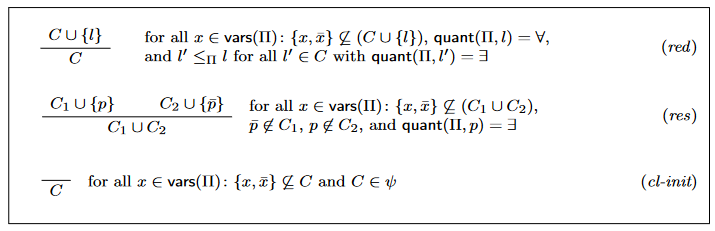
\includegraphics[width=1\textwidth]{../graphics/q-res-proof.png}
\caption{Q-resolution proof system from \cite{handbook}.}
\label{pre:qres}
\end{figure}

\begin{example}
    $\exists y \forall x z \exists p (y \lor x \lor z) \land p$ by applying only (red) for $(y \lor x \lor z)$ we get $(y \lor x)$ because $l \leq_\Pi x$ and $p$ is not in the clause, also we can get $(y \lor z)$ because $z$ needs to be higher than existential variables and ignore the universal quantified variables, in plus, if we apply it repeatedly we can also get $(y)$.
\end{example}

\textrosu{why tautology so probebatic}
\stodo{how to check sound of a red, with semantics?}

\begin{example}
    $\forall x y \exists z (x \lor z) \land (y \lor \overline{z})$ with (res) on those 2 clauses, we get $(x \lor y)$.
\end{example}

\begin{example}
    In this example we will apply the rules to get a refutation for $\forall x_1 x_2 \exists y (x_1 \lor x_2 \lor \overline{y}) \land (y \lor \overline{x_1}) \land (y \lor \overline{x_y}) \land y \land (x_1 \lor \overline{x_1})$. Firstly we apply (cl-init) where we get $(x_1 \lor x_2 \lor \overline{y}) \land (y \lor \overline{x_1}) \land (y \lor \overline{x_y}) \land y$ without last clause because that is a tautology. On the first and last clause we can apply (res) and get $(x_1 \lor x_2)$. On $(x_1 \lor x_2)$ we apply twice (red) and get the empty clause, $\bot$. Thus, our formula is false and have a proof in Q-resolution proof system.
\end{example}
\subsection{QRAT Proof System}

The main objective of this work, is to provide a QRAT proof for an input PCNF, where QRAT is derived from the quantified circuit of the PCNF. Thus, we dedicate this section to provide the prerequisite for a QRAT proof.

The QRAT proof system \stodo{...}

\begin{definition}[Outer Resolvent \cite{handbook}]
    The \textbf{outer resolvent} of clauses $C \lor l$ and $D \lor \overline{l}$ on literal $l$ w.r.t. qunatifiers $\Pi$ is:
    \[ \text{OR}(\Pi, C \lor l, D \lor \overline{l}, l) = C \cup \{k \mid k \in D, k \leq_\Pi l, k \not= \overline{l}\}, \text{for quant}(\Pi, l) = \exists,  \]
    and:
    \[ \text{OR}(\Pi, C \lor l, D \lor \overline{l}, l) = (C \backslash \{l\}) \cup \{k \mid k \in D, k \leq_\Pi l, k \not= \overline{l}\}, \text{for quant}(\Pi, l) = \forall.  \]

\end{definition}

\begin{example}
    Given $\Pi = \forall x_1 x_2 \exists y_1y_2 \forall x_3 x_4$.
    
    For $C = (x_2 \lor x_4 \lor y_1), D = (x_1 \lor x_3 \lor \overline{y_1})$, with the existential quantifier $y_1$ as the pivot, we get OR $=(x_2 \lor x_4 \lor y_1 \lor x_1)$.

    For $C = (y_1 \lor y_2 \lor x_1), D = (x_2 \lor \overline{x_1})$, with the universal quantifier $x_1$ as the pivot, we get OR $=(y_1 \lor y_2 \lor x_2)$.
\end{example}

\begin{definition}[Implies via Unit Propagation \cite{handbook}]
    A propositional formula $\psi$ \textbf{implies via unit propagation} a clause $C$, denoted by $\psi \vdash_1 C$, 
    
    iff applying unit propagation on $\psi \land \overline{C}$ we can derive empty clause $\bot$. 
\end{definition}

\begin{example}
    Given $\psi = (\overline{a} \lor b) \land (\overline{c} \lor d) \land (\overline{c} \lor \overline{d})$ and the clause $C = (a \lor b)$. \stodo{continue}
\end{example}

\begin{definition}[QRAT \cite{handbook}]
    A clause $C$ has \textbf{QRAT on literal} $l \in C$ w.r.t. QBF $\Pi\psi$, iff for all $D \in \psi$ with $\overline{l} \in D$:
    \[ \psi \vdash_1 \text{OR}(\Pi, C, D, l). \]
\end{definition}

\begin{example}
    \stodo{continue}
\end{example}

With the QRAT definition in place, in order to make use of it we use the following theorems, from \cite{qrat}, that help us to transform a QBF in a satisfiable equivalent QBF:

\begin{theorem}[QRAT for existential \cite{qrat}]
    Given a QBF $\phi = \Pi.\psi$ and a clause $C \in \psi$ with QRAT on existential literal $l \in C$ w.r.t. QBF $\phi' = \Pi'.(\psi \backslash \{C\})$, where $\Pi'$ is adapted for $(\psi \backslash \{C\})$. Then $\phi$ and $\phi'$ are equisatisfiable. 
\end{theorem}

\begin{theorem}[QRAT for universal \cite{qrat}]
    Given a QBF $\phi = \Pi.\psi$ and a clause $C \in \psi$ with QRAT on universal literal $l \in C$ w.r.t. QBF $\Pi.(\psi \backslash \{C\})$. Then $\phi$ and $\Pi.(\psi \backslash \{C\} \cup \{C \backslash \{l\}\})$ are equisatisfiable. 
\end{theorem}

\stodo{speak whats with them}

\stodo{EUR}

\stodo{the proof system cheking}
\subsection{QCDCL}

In this section, we will present an algorithm that can solve a QBF instance, with the underlying proof of the solution given in the Q-Resolution framework. The quantified conflict driven clause learning is the quantified version for the CDCL used for SAT solving. For the propositional problem in the satisfiable case it's enough to have an assignment, thus the CDCL algorithm tries to guess an assignment that evaluates the input to true, but in case the decisions result in a false formula, the procedure tries to derive a clause that minimize the search space. Similarly, in QCDCL we learn clauses to prune the search space of falsifying assignments, and learn cubes for running the satisfying assignment, \cite{handbook}.

\textrosu{Propozitie sa introduc ce urmeaza.}

\begin{figure}[H]
\centering
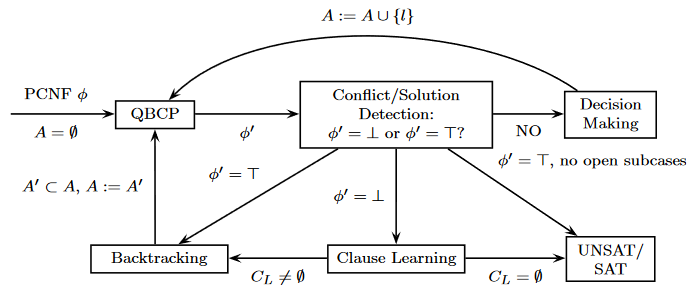
\includegraphics[width=1\textwidth]{../graphics/qcdcl-flowchart.png}
\caption{Flowchart of QCDCL from \cite{handbook}.}
\end{figure}

\stodo{cum merge figura}

\begin{definition}[Unit literal detection \cite{handbook}]
    A clause $C \in \phi$ is \textbf{unit} iff $C$ contains one literal, and the literal is existential quantified. That literal is also called a \textbf{unit literal}. \textbf{Unit literal detection} applied to a QBF collects all unit clauses in the QBF.
\end{definition}

\begin{example}
    Let our formula be $\forall x_1x_2 \exists y_1 \forall x_3 \exists y_2 (x_1 \lor x_2) \land x_3 \land y_1 \land \overline{y_2}$. The unit literal detection gives us $\{y_1, \overline{y_2}\}$.
\end{example}

\begin{definition}[QBCP \cite{handbook}]
    Given a PCNF $\phi$ and the empty assignment $A = \{\}$. We apply the following:
    \begin{enumerate}
        \item Apply universal reduction (UR) on $\phi[A]$ to get $\phi[A]'$.
        \item Apply unit literal detection (UL) on $\phi[A]$ and append the result to $A$.
        \item Repeat from 1. Stop if $A$ haven't changed, or the formula is true or false.
    \end{enumerate}
\end{definition}

\begin{example}\label{example:qbcp}
    Given $\phi = \forall x_1 x_2 \exists y (x_1 \lor x_2 \lor \overline{y}) \land (y \lor \overline{x_1}) \land (y \lor \overline{x_y}) \land y$ we apply QBCP, we start with $A$ empty:
    \begin{itemize}
        \item We cannot apply UR.
        \item From $\phi[]$ with UL, we get $A = \{ y \}$.
        \item $\phi[y] = \forall x_1 x_2 (x_1 \lor x_2)$, we apply UR on $x_2$, and we get $\phi[y] = x_1$
        \item We cannot apply UL, because no existential literal is present.
        \item By applying UR, we get $\phi[y] = \bot$. Thus, we stop.
    \end{itemize}
\end{example}

\stodo{the scope of the work is not the solver but to derive a prove briefly bla bla}
Using the previous example \ref{example:qbcp}, 

\textrosu{how a proof would look like for $\exists xy (\neg x \lor y)$ after assign of $x$}
\subsection{QDIMACS Format}
\subsection{QCIR Format}

\section{QCIR Reconstruction Certification}

In this chapter, we present the main aim of the work: quantified circuit reconstruction certification. Given a QBF $\phi$ in PCNF and a QCIR converter, our goal is to verify that the output of the converter is equisatisfiable with the given input. Restricting our approach only for the false instances of QBF, in order to check the satisfiable equivalence we propose the following solution: after we apply the converter, and get the formula $\phi_\text{QCIR}$, we can reconstruct a refutation proof for $\phi$ from $\phi_\text{QCIR}$ refutation proof. This way, with the initial proof reconstruction, we can reassure the sound of the QCIR converter.

In the following, we assume that the input formula is false, and a QCIR converter gives a circuit that uses variables from the input without addition of other new variables.

In the first section \stodo{write after sections done}

\subsection{Certification procedure}

\begin{algorithm}[H]
\caption{Procedure for initial proof reconstruction from QCIR conversion.}\label{alg:cap}
\begin{algorithmic}[1]
\Require False PCNF: $\phi$, QCIR converter procedure: \textsc{QcirConv}
\Ensure QRAT refutation proof P for $\phi$
\Procedure{GetInitialProof}{$\phi$, \textsc{QcirConv}}
\State $\phi_\text{QCIR} \gets$ \Call{QcirConv}{$\phi$}
\State $\phi_\text{Tseitin} \gets$ \Call{TseitinOfQcir}{$\phi_\text{QCIR}$}
\State $P_\text{Q-Res} \gets$ \Call{QBFSolver}{$\phi_\text{Tseitin}$}
\State $P_\text{QRAT} \gets$ \Call{QresToQrat}{$P_\text{Q-Res}$}
\State $P_\text{Initial-QRAT} \gets$ \Call{InitialQratReconstruction}{$\phi, \phi_\text{Tseitin}, P_\text{QRAT}$}
\State \Return $P_\text{Initial-QRAT}$
\EndProcedure
\end{algorithmic}
\end{algorithm}

In algorithm \ref{alg:cap} s

\subsection{tseitin transform}
\subsection{Getin qrat proof}
\subsection{verification}
\section{Implementation}
% \section{Experiment}
% \section{Conclusion}

\bibliographystyle{ieeetr}
\bibliography{biblio.bib}

\end{document}